


%
% How to fix the Underfull \vbox badness has occurred while \output is active on my memoir chapter style?
% https://tex.stackexchange.com/questions/387881/how-to-fix-the-underfull-vbox-badness-has-occurred-while-output-is-active-on-m
%

% ---

\lang
% {\chapter[Page not filled]{Since this page is not being completely filled, it is generating the bottom bottom of the page}}
% {\chapter[Página não gerada]{Como esta página não está sendo completamente preenchida, ele está gerando a caixa inferior inferior da página}}
% ---


% Multiple-language document - babel - selectlanguage vs begin/end{otherlanguage}
% https://tex.stackexchange.com/questions/36526/multiple-language-document-babel-selectlanguage-vs-begin-endotherlanguage
\begin{otherlanguage*}{brazil}

\chapter{Manual de configuração da LTI Beecrowd no Moodle}
\label{manual:config-lti}

O administrador do Moodle deve configurar a LTI do Beecrowd.


\begin{enumerate}
    \item Acessar o moodle com uma conta de administrador
    \item Selecionar a opção: \textbf{Plugins}

    \begin{figure}[h!]
        \centering
            
\includegraphics[scale=0.45]{pictures/apendices/apendice_a_1.png}
    \end{figure}

    \item Em Activity Modules, selecionar \textbf{External tool} -> \textbf{Manage tools}

    \begin{figure}[h!]
        \centering
            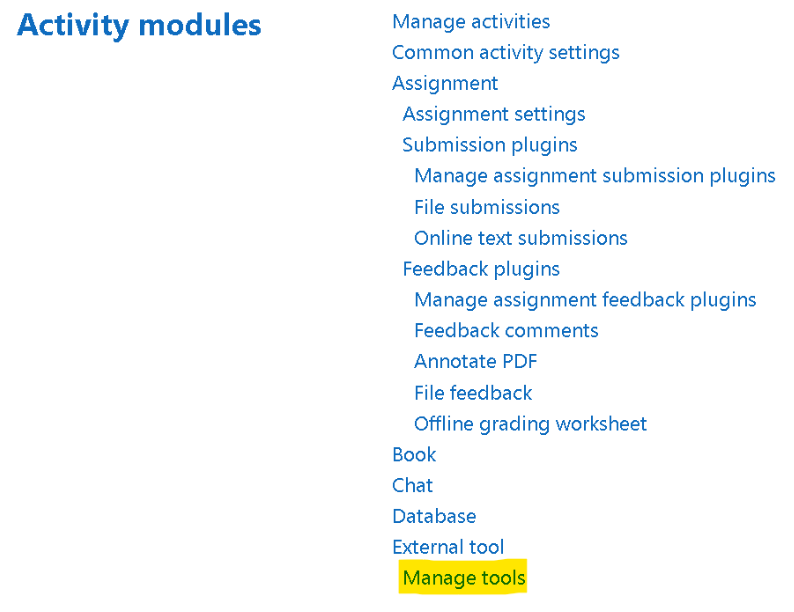
\includegraphics[scale=0.5]{pictures/apendices/apendice_a_2.png}
    \end{figure}

    \item Selecionar a opção \textbf{configure a tool manually}

    \begin{figure}[h!]
        \centering
            
\includegraphics[scale=0.4]{pictures/apendices/apendice_a_3.png}
    \end{figure}

    \item Na página a seguir, preencher os campos conforme abaixo:\\

    Tool name: \textit{beecrowd} \\
    Tool URL: \textit{https://api.beecrowd.com/} \\
    Tool description: \textit{beecrowd LTI1.3 moodle integration} \\
    LTI version: \textit{LTI 1.3} \\
    Public key type: \textit{Keyset URL} \\
    Public keyset: \textit{https://api.beecrowd.com/lti/jwks} \\
    Initiate login URL: \textit{https://api.beecrowd.com/lti/login} \\
    Redirection URI(s): \textit{https://api.beecrowd.com/lti/launch} \\
    Custom parameters: “Manter vazio” \\
    Tool configuration usage: \textit{Show in activity chooser and as a preconfigured tool} \\
    Default launch container: \textit{New window} \\
    Supports Deep Linking (Content-Item Message): \textit{“Assinalar o check box”} \\
    Content Selection URL: \textit{https://api.beecrowd.com} \\
    
    Icon URL: \textit{https://moodle.beecrowd.io/pluginfile.php/15/course/summary/lgo.png} \\
    Secure icon URL: \textit{https://moodle.beecrowd.io/pluginfile.php/15/course/summary/lgo.png} \\
    
    \textbf{Services} \\
    IMS LTI Assignment and Grade Services:  \textit{Use this service for grade sync and column management} \\
    IMS LTI Names and Role Provisioning: \textit{Use this service to retrieve members' information as per privacy settings} \\
    Tool Settings: \textit{Use this service} \\
    
    \textbf{Privacy} \\
    Share launcher's name with tool: \textit{Always} \\
    Share launcher's email with tool: \textit{Always} \\
    Accept grades from the tool: \textit{Always} \\
    Force SSL: “Não assinalar” \\
    
    \textbf{Miscellaneous} \\
    Default organisation ID:  \textit{Site hostname} \\
    Organisation ID: “Manter Vazio” \\
    Organisation URL: \textit{https://beecrowd.com/} \\
    

    \item Após configurar as informações acima, você deve enviar para o Beecrowd a captura de tela da seguinte tela (exemplo na foto abaixo) através do botão de e-mail com os dados que eles devem inserir na parte deles para estabelecer a comunicação:
    
    \begin{figure}[h!]
        \centering
            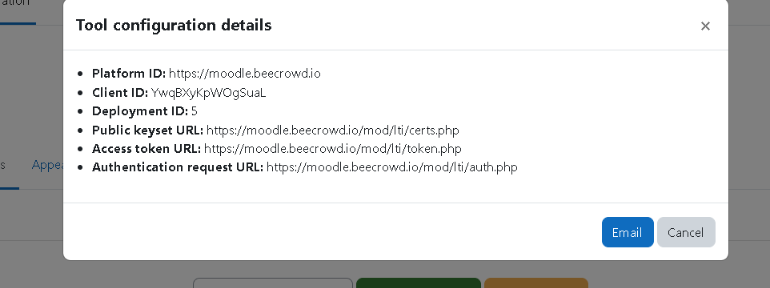
\includegraphics[scale=0.4]{pictures/apendices/apendice_a_5.png}
    \end{figure}
    
    \item Será exibida uma página de autorização. Basta preencher o email e aguardar a aprovação. Uma vez feito, é necessário recarregar a sessão e iniciar os testes novamente.

    \begin{figure}[h!]
        \centering
            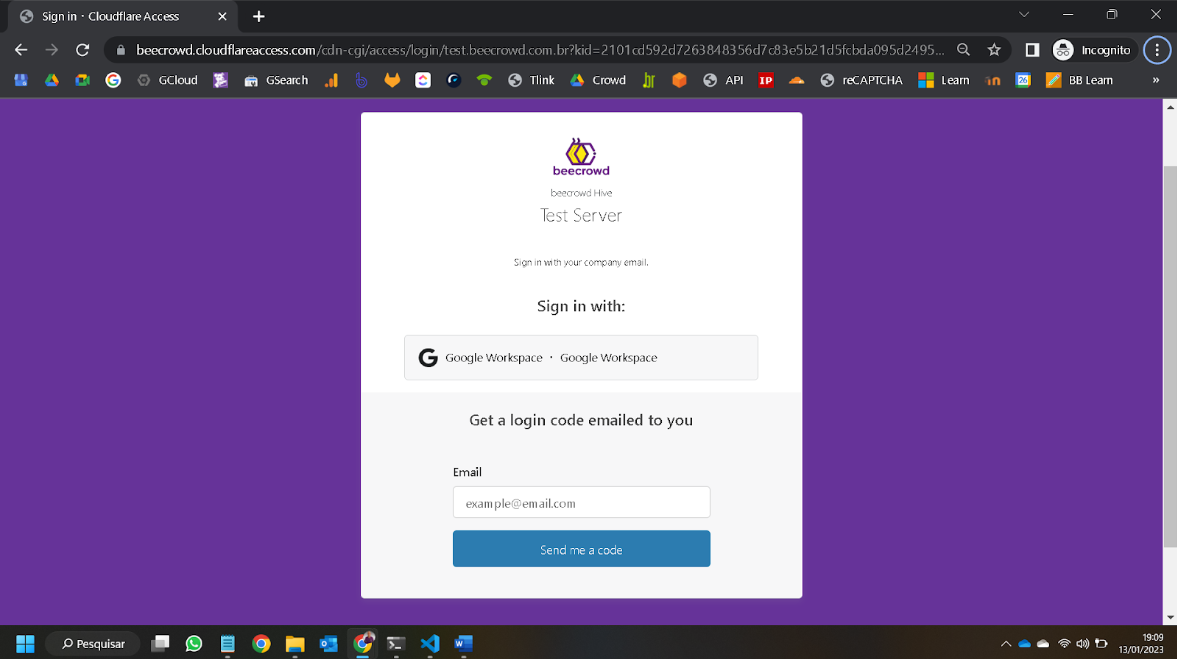
\includegraphics[scale=0.4]{pictures/apendices/apendice_a_6.png}
    \end{figure}

\end{enumerate}

\end{otherlanguage*}


